\ifx\wholebook\relax\else
\input{../Common.tex}
\input{../macroes.tex}
\begin{document}
\fi


%\newcommand{\scrref}[1]{Script~\ref{#1}\xspace}
%\newcommand{\mthref}[1]{Method~\ref{#1}\xspace}
%\newcommand{\clsref}[1]{Class~\ref{#1}\xspace}

\chapter{Implementing Joe the Box}\label{ch:Joe}

\begin{chapterfigure}
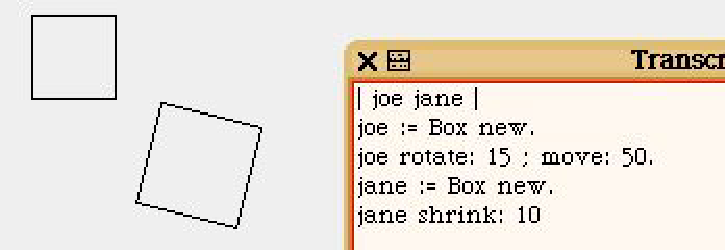
\includegraphics{joeTheBoxHeader}
\end{chapterfigure}

@@Should we change the class definition template@@



In this chapter you will program your first class, the class \ct{Box}. 
Doing so you will learn how to describe the behavior and the state of
objects.  We start with a first implementation that we later refine. 
This first class is one of the first example used to teach
object-oriented concepts to novices by researchers that invented
object-oriented programming.

\section{Box's Behavior and State}\label{sec:firstimplementation}

A box has the following behavior, it knows how to draw itself, move to
a given distance, move to a given point, rotate, grow and shrink.  A
typical scenario is described by \scrref{scr:scenario}.  A graphical
result is shown by the first figure of the chapter above.

\begin{scriptwithtitle}{A typical Box scenario}\label{scr:scenario}
| joe jane |
joe := Box new.
joe rotate: 15.
joe grow: 100.
joe move: 10@10.
joe moveTo: 150@200. 
jane := Box new.
jane move: 30@-30.
jane shrink: 40.
jane rotate: 45
\end{scriptwithtitle}
    
It is worth to spend some time looking at \scrref{scr:scenario}.  It
shows that while at the first glance the scripts may look similar ot the turtle messages they
are not.  From an object point of view, there is difference between
asking a turtle to draw a square as shown in \charef{cha:} and asking
a box to draw itself.  The methods and the arguments that they require
are different.  Here a box knows how to grow, shrink and rotate.

Before starting programming, we have to analyze the behavior of a box 
to imagine a possible way to program it. Here is the 
behavior a box should have. A box should know how to:

\begin{itemize}
\item draw itself at a given location. When a new box is created it 
 automatically displays itself. 
\item move to a given location (method \ct{moveTo: aPoint}).
\item rotate from a given angle (method \ct{rotate: anInteger}).
\item translate from a certain distance (method \ct{move: aPoint}).
\end{itemize}



It is fundamental to start by looking at objects from their
\emph{behavior}.  An object is a behavioral entity, \emph{i.e.,} an
entity reacting to messages.  A similar behavior can be implemented by
different manners so it is crucial not to start to think in terms of
the internal structures that may represent the object but in
terms of the essence of the object, its \emph{behavior}.
  
\begin{teacher}   
Note the way we phrase the sentences describing box actions:  we do
not say the box is displayed but it displays itself.  We always use
the active form where the subject is the object itself.  Considering
the object as a living being is a good way to think in an
object-oriented manner.  Imagine talking about an animal or a person
you will say that the person acts and not is acted by others.  
\end{teacher}


\paragraph{From behavior to state.} Now from this description of the
box's behavior, we should imagine a possible state for a box that
could be used to implement the wished behavior.  As this example and
the concept of box are familiar, we propose that boxe state is
represented by a size, a position and a tilt.

In fact any box will be represented by such a triplet (size, position
and tilt) but each given object will have its own triplet values.  For
example, the box referenced by the variable \ct{joe} in
~\scrref{scr:scenario} has its \emph{own} state, \emph{i.e.,} its own
size, position, and tilt.  In the same way the box \ct{jane} has a
\emph{similar} state because it is also a box created from the class
\ct{Box} too but it has its own state which may or not equal to the
one of \ct{joe}.  When the state of one given box changes it does not
change the state of the other boxes.  This situation is illustrated by
the first figure of this chapter.  If this aspect is not clear we
suggest you to (a) read \charef{ch:objects} and (b) create the class
\ct{Box}, inspect two instances and modify their states.



\section{Defining the class \ct{Box}}

To create a class we use a dedicated browser called the system browser
\index{system browser} or class browser \index{class browser} as presented in \charef{cha:Browsers}.  To open such a browser, bring up the default menu and chose the menu item \menu{open...} and the item \menu{browser} (or use the \shortcut{b}).


%\begin{figure}
%\begin{center}
%\includegraphics[]{newCategory}
%\caption{Bring up the menu over the leftmost pane of the browser and 
%select the add item choice to create a new class category.   
%\label{fig:newBoxCategory}}
%\end{center}
%\end{figure}

\begin{figure}
\begin{center}
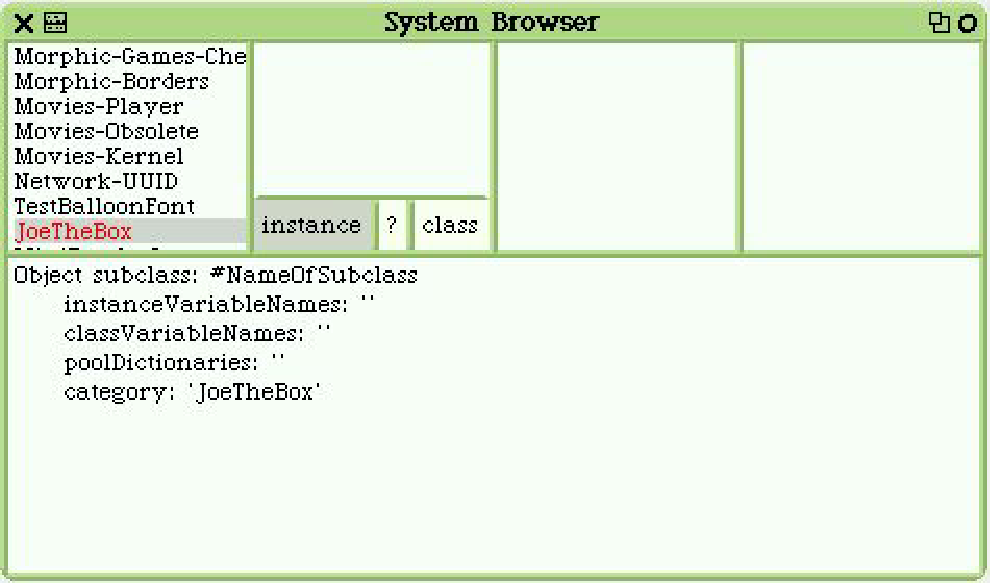
\includegraphics[width=8cm]{boxCategory}
\caption{The browser shows you that a new class has been created by displaying
it in the second pane from the left. \label{fig:boxCategory}}
\end{center}
\end{figure}

To create a class, create first a new category (which represents a
folder for all the classes we will create related to this small
project) by selecting the item \menu{add Item} of the menu associated with the
leftmost pane of the browser (as explained in~\charef{cha:browser}).  Name
it for example \ct{JoeTheBox}.  When you select the newly created category,
the system displays a template to help you defining a new class (see
~\clsref{cls:template} and the figure~\ref{fig:boxCategory}).

\begin{classdef}\label{cls:template}
Object subclass: \#NameOfClass
   instanceVariableNames: 'instVarName1 instVarName2'
   classVariableNames: 'ClassVarName1 ClassVarName2'
   poolDictionaries: ''
   category: 'JoeTheBox'
\end{classdef}




\begin{figure}
\begin{center}
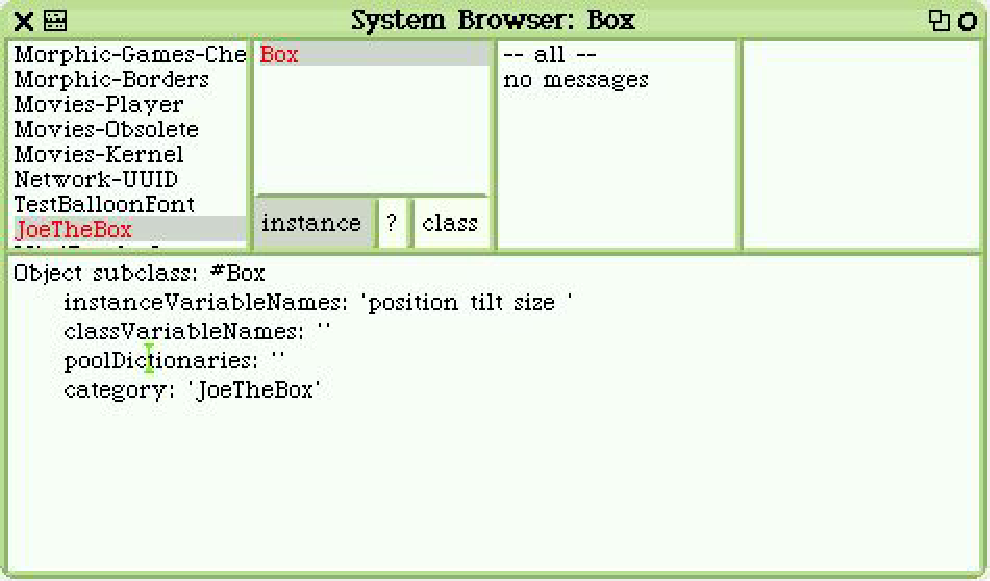
\includegraphics[width=8cm]{classBoxCreated}
\caption{The browser shows you that a new class has been created by displaying
it in the second pane from the left. \label{fig:classBoxCreated}}
\end{center}
\end{figure}


Modify the proposed template to obtain
~\clsref{cls:boxDefinition} and in the bottom pane bring the
menu and choose the menu item \menu{accept}.  Now the class exists. 
The system shows you that the class is defined by displaying it in the
second pane as shown in figure~\ref{fig:classBoxCreated}.  Using the
terminology used in other programming languages we can say that the
class has been \emph{compiled}.  This means that we could already
create instances of this class, even if now this is not really useful
since they do not have any specific behavior.

\begin{classdef}\label{cls:boxDefinition}
Object subclass: #Box
   instanceVariableNames: 'position size tilt '
   classVariableNames: ''
   poolDictionaries: ''
   category: 'Joe The Box'
\end{classdef}
	
Here are some explanations about the class definition \ref{cls:boxDefinition}: A box is a
simple object.  Hence, it is a subclass \ct{Object}\index{\ct{Object}}
(The concept of subclass and inheritance is explained
\charef{cha:inheritance}).  The internal state of box instances, such
as the boxes \ct{joe} and \ct{jane}, is represented by instance
variables \index{instance variables} of the class \ct{Box}.  So line 2
we specify that the class \ct{Box} has three instance variables by
given their respective names.  Here the class \ct{Box} has the
instance variables \ct{position}, \ct{size}, and \ct{tilt}.  This
indicates to the class \ct{Box} to create instances having three
values representing the box's state.  As shown by
\clsref{cls:boxDefinition} we empty the other parts of the templates
because they are irrelevant for now.



\important{
A class acts as an object factory, an instance model, or a mould. 
The instance variables describe the state that  the instances created 
by the classes will have. Each instance of the class will have the structure 
described by the class but filled with \emph{its own} values.}


Instances have their own state but it follows the description given by the class. Two instances of the same class can have different values for the same instance variable but they cannot have a different number of instance variables. 

\begin{teacher}
The \emph{factory} or mould metaphor is really useful to explain the difference between classes
and instances. Here, the class \ct{Box} describes and creates boxes of different size, position and tilt but all have these three characteristics.\end{teacher}

\section{Initializing Instances}\label{sec:initializeInstance}

Once the class is defined, create and inspect one of its instances by
executing~\scrref{scr:box} or by using an inspector (see~\charef{ch:usingInspector}).  The
figure~\ref{fig:uninitializedBox} shows an inspector on a \ct{Box}
instance.  All the instance variables have \ct{nil}\index{nil} as
value.  Indeed, when an instance is created by invoking the method
\ct{new}\index{new} on a class, the \emph{default} behavior of the
class is to return an \emph{uninitialized}
instance\index{initialization}.  Uninitialized means that all the
instance variables of the newly created instances have no value.  To
represent the \emph{no value} concept, Smalltalk  uses the special object 
\ct{nil}\footnote{Nil comes from the latin nihil which means
nothing.}.  That's why the instance variables of the inspected box
have all as value \ct{nil}.

\begin{scriptwithtitle}{Inspecting a box}\label{scr:box}
Box new inspect
\end{scriptwithtitle}

\begin{figure}
\begin{center}
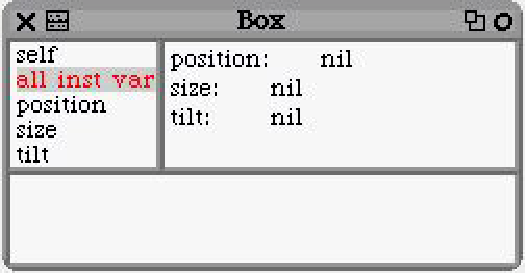
\includegraphics[width=5cm]{unintializedBox}
\caption{Inspecting a \emph{non initialized box}: all its instance variables 
are empty, \emph{i.e.,} having \ct{nil} as value.\label{fig:uninitializedBox}}
\end{center}
\end{figure}

Having uninitialized values is not really good because methods may not
work or have to test if the variables have been correctly initialized. 
But even then this is not satisfactory because if an instance variable
is not initialized it is difficult to know the value to initialize it. 
In fact the best solution is to initialize the instance as soon as it
is created.  



For that purpose we specialize the method \ct{initialize} that sets up
a default state for a box.  The method \ct{Box>>initialize} is
automatically invoked by the method \ct{new} on newly created
instances.  This method sets the instance variables values.  Once this
method defined, in the bottom pane of the inspector evaluate the expression 
\ct{self initialize}. If you closed the inspector or want to convince you that the method \ct{initialize}
is invoked when a new instance is created,  reuse \scrref{scr:box} to check that the created
instance is now well initialized. In both cases, you should obtain a situation 
similar to the one described by the figure~\ref{fig:initializedBox}.

\begin{method}\label{mt:boxInitialize}
Box>>initialize
   "A box is initialized to be in the center of the screen, with 
   50 pixels size and 0 tilt"
   
   size := 50.
   tilt := 0.
   position := World bounds center
\end{method}

\begin{figure}
\begin{center}
\includegraphics[width=5cm]{boxInitialized}
\caption{Inspecting an \emph{initialized box}: all its instance variables 
contains some values coherent with their role.\label{fig:initializedBox}}
\end{center}
\end{figure}

\begin{readerNote}
The fact that the \ct{new} method automatically call the \ct{initialize}
method is a little extension we added into \sq.  It may happen that
such an extension will be included into \sq at the time you will read
this book.  In any case the plain \sq solution to this problem is
explained in \charef{ch:InstanceInitialization} so that you can
understand and program in \sq without our little extension.
\end{readerNote}







\section{Accessing Instance Variables}
The method \ct{initialize} above illustrates an important aspect of
the object model of \sq.  The instance variables are accessible from
the methods as if they were defined in the method body. For example, 
we are assigning \ct{50} in the instance variable \ct{size}. The instance 
variable \ct{size} is accessible from any method of the class \ct{Box}.

Contrary to the \index{local variables}  of a
script  (\ct{| caro | for example}) which do not exist after the script execution, instance
variables last the complete object life-time.  We propose you some
experiments to really understand this phenomena below.  Note that this
behavior is not new, we used it constantly with the turtle.  For
example, we changed the direction of the turtle using the method
\ct{north} which was somehow changing the internal turtle state representing its direction, then later used the direction to perform some other actions.

We propose you to do some experiments to really understand this notion. 
Define the methods \ct{size} (\mthref{mt:size}) which returns the value 
of the instance variable \ct{size} and \ct{size: anInteger} 
(\mthref{mt:sizeAssign}) which changes the value of 
the instance variable \ct{size} to be the one specified as argument. Such a kind of methods are called \emph{accessor} methods because they only get and set information in instance variables. 
The code \ct{\^size} returns the value of the instance variable size.

\cadre{In \sq to return a value, use the character \^\ followed by the 
expression whose value has to be returned.}



\begin{method}\label{mt:size}
Box>>size

   ^size
\end{method}

\begin{method}\label{mt:sizeAssign}
Box>>size: anInteger

   size := anInteger
\end{method}


Now execute \scrref{scr:instanceVarLife} and use the menu item
\menu{print it} to get the results we present in  \scrref{scr:instanceVarLife} using \emph{returns}. If you have an inspector opened
on a box instance, you can also execute the messages \ct{self size}, \ct{self size: 10} in the bottom left part of the inspector. Perform some other experiments to prove yourself that you understand.

\begin{scriptwithtitle}{Instance variables 
life-time}\label{scr:instanceVarLife}
| joe jane |
joe := Box new.
joe size. \emph{returns} \ct{50}
joe size: 10.
joe size. \emph{returns} \ct{10}
joe size: 20.
joe size. \emph{returns} \ct{20}
joe size: joe size + 5.
joe size. \emph{returns} \ct{25}
jane := Box new.
jane size. \emph{returns} \ct{50}
\end{scriptwithtitle}


Now that you understand better instance variables, you should notice that instance variables are private information of objects so creating \emph{accessor} methods like the methods\ct{size} and \ct{size:} above that only access and return the value of an instance variable open the privacy of instances. We say that the break the encapsulation of the object data. We will discuss in \charef{cha:accessor} the use of accessors\index{accessor} methods.

In summary we have: 

\cadre{Instance variables are accessible to all the methods of a class. 
Instance variables last the same life-time than the object to which 
they belong to.}

\cadre{In \sq, instance variables cannot be accessed from outside of 
an object. Instance variables are only accessible from the methods of 
the class that define them.}

\section{Drawing a Box and Other Operations}
Now that we initialize a newly created box using the method
\ct{initialize}, we are in position to define methods without been
worried about the initialization of instance variables.  

During your experiments you may want to clear the
screen\index{clearing screen}.  Use the \scrref{scr:clearingScreen}
for that purpose.

\begin{scriptwithtitle}{Clearing the screen}\label{scr:clearingScreen}
World clearTurtleTrails
\end{scriptwithtitle}

\paragraph{Method \ct{draw}.} We define the method \ct{draw} that uses a
turtle but we hide it as shown by \mthref{mt:draw}.  We create a
method, put it at the right position of the box, set the direction of
the turtle to the tilt of the box, use the black color and then draw a
square of the box size.

\begin{method}\label{mt:draw}
Box>>draw
   "Draw the receiver position in black"
   "Box new initialize draw"
	
   | aTurtle |
   aTurtle := Turtle new hidden.
   aTurtle jumpAt: position.
   aTurtle turnRight: tilt.
   aTurtle penColor: Color black.
   4 timesRepeat: [aTurtle go: size. 
                  aTurtle turnLeft: 90]
\end{method}


\begin{figure}
\begin{center}
\includegraphics[width=12cm]{inspectedBoxDraw}
\caption{A problem with the \ct{grow:} method. The box is not erased when it changes its size.\label{fig:drawingBox}}
\end{center}
\end{figure}

As soon as the method is defined and all the methods it calls exist, it is possible to invoke it.
Test the method by executing the code \ct{self draw} into the bottom pane of an inspector in a similar way than shown in figure~\ref{fig:drawingBox}, or by executing \scrref{scr:draw}.

\begin{scriptwithtitle}{sending the message draw to a box}\label{scr:draw}
| joe jane |
joe := Box new.
joe draw
\end{scriptwithtitle}




\begin{exercise}
Up until now, creating a new box did not displayed it.  Change the
method \ct{initialize} so that any new box is automatically displayed.
\end{exercise}


\paragraph{Method grow:} The method \ct{grow: anInteger} makes the box
growing of a certain size and redraw itself to reflect this size
change.  Propose a definition and  use the inspector or dedicated scripts to tests your method. 

\begin{method}\label{mth:grow}
Box>>grow: anInteger 
   "grow the receiver's size from increment"
   
    size := size + anInteger.
    self draw
\end{method}


We propose the definition~\ref{mth:grow} for the method \ct{grow:}.
However, try \scrref{scr:growProblem} to see that we have a problem and 
propose a solution.


\begin{scriptwithtitle}{Problem with the first \ct{grow:} 
method.}\label{scr:growProblem}
| joe |
joe := Box new.
joe grow: 20.

joe grow: 40
\end{scriptwithtitle}

The problem we have is that the turtle grows and redisplay itself 
well, but it does not remove the previous box shape. To solve that 
problem we propose you to define a method named \ct{undraw} which 
is similar to the draw method except that it draw the box using a 
transparent color (\mthref{mt:undraw}).

\begin{method}\label{mt:undraw}
Box>>undraw
   "erase the receiver"
   
   | aTurtle |
   aTurtle := Turtle new hidden.
   aTurtle jumpAt: position.
   aTurtle turnRight: tilt.
   aTurtle penColor: \textbf{Color transparent}.
   4 timesRepeat: [aTurtle go: size.
                  aTurtle turnLeft: 90]
\end{method}

Now that the method \ct{undraw} is defined, the method \ct{grow:} should 
call it before anything else as shown by \mthref{mt:goodGrow}.

\begin{method}\label{mt:goodGrow}
Box>>grow: increment 
   "grow the receiver's size from increment"

   \textbf{self undraw}.
   size := size + increment.
   self draw
\end{method}


To be able to execute the script we presented at the beginning of the chapter, implement the methods
\begin{itemize}
\item  \ct{move: aPoint} which translate the box 
from a distance in x and y specified as a point. 
\item \ct{moveAt: aPoint} which move the box to the specified point.
\item \ct{rotate: anInteger} which rotates the box of a given angle. 
\item \ct{grow*: anInteger} and \ct{shrink*: anInteger} 
that make grow and shrink the receiver by a given factor.
\end{itemize}







\section{Limiting Duplication}\label{sec:}
The methods \ct{draw} (\mthref{mt:draw}) and \ct{undraw}
(\mthref{mt:undraw}) are nearly the same except for the color of the
turtle.  This is not really good, since every times we will change one
method we will have to change the other and there is chance that we
forgot. Note that on this really simple example this is not really a
problem but we want to show you a good principle.

Propose a solution to this problem. The idea is that to avoid
duplication, the methods \ct{draw} and \ct{undraw} can call a third
method with the color of the pen as argument. We could named this
method \ct{drawWithColor:}. Try to implement such a method before
reading the solution.

The \ct{drawWithColor: aColor} (\mthref{mt:drawWithColor}) shows a
possible implementation, it factors out the duplicated code. Now
change the methods \ct{draw} and \ct{undraw} to call this method with
the right argument.

\begin{method} \label{mt:drawWithColor}
Box>>drawWithColor: aColor 
   "Draw the receiver using a given color"
	
   | aTurtle |
   aTurtle := Turtle new hidden.
   aTurtle jumpAt: position.
   aTurtle turnRight: tilt.
   aTurtle penColor: \textbf{aColor}.
   4 timesRepeat: [aTurtle go: size.
                  aTurtle turnLeft: 90]
\end{method}

\comment{\begin{method}
Box>>draw
   "draw the receiver in black"
   
   self drawWithColor: Color black
\end{method}

\begin{method}
Box>>undraw
   "erase the receiver"
   
    self drawWithColor: Color transparent
\end{method}}

In general we should avoid as much as possible to have duplicated
code.  This is not a problem to duplicate code for a small experiment.
However, if you want to keep the code always think that you should
create other method to share and reuse the duplicated code. Creating
one or several methods to factor the duplicated code is a good trick
to cure duplicated code.

\cadre{Avoid duplicated code. Refactor the duplicated code by calling 
a method representing the duplicated code.}




\section{Looking at Alternate  Designs}
We said that the implementation we proposed is one of the multiple
ways of implementing the behavior of the \ct{Box} class. In this
section we want to look at other possible implementations.  First let
us analyze the current implementation.  The class \ct{Box} has its own
state via the instance variables \ct{tilt}, \ct{position}, and
\ct{size} then gives a part of its state to a turtle, its tilt and 
position.  The \ct{Box} class uses the \ct{Turtle} class to realize
its behavior.  This is a common practice where a class do not repeat
behavior but reuse the behavior of an existing class.

We used the class \ct{Turtle} because it was familiar to us.  However,
another class, the class \ct{Pen} could have been a possible candidate
too.  Look at the class \ct{Pen} and change the method
\ct{drawWithColor:} to use it instead of \ct{Turtle}.  What is
important is that the interface proposed by the class \ct{Box} should
not changed.  We are changing the internal implementation of the class
\ct{Box }but this should not change its behavior.

Now if we look carefully we see that the turtle or the pen instance
are created every time the box is draw and undraw.  In addition the
state of the box is systematically copied to the turtle state then
lost because a turtle is recreated and the previous one is lost.  One
idea would be to use a turtle as representing part of the box state.
Indeed a turtle has also a position and a tilt.  

Define the class \ct{BoxT} as shown below in
\clsref{cls:alternateBoxDefinition} and reimplement some of the box's
methods to convince you that this is possible. This solution has the
advantages that less objects are created, less state is copied from
the box to the turtle and as drawbacks that the class \ct{Box} is tied
with the class \ct{Turtle}.

\begin{classdef}\label{cls:alternateBoxDefinition}
Object subclass: #BoxT
   instanceVariableNames: 'size turtle'
   classVariableNames: ''
   poolDictionaries: ''
   category: 'Joe The Box'
\end{classdef}


To help you we show two methods, \mthref{mt:boxAlternateInitialize} and 
\mthref{mt:alternateDrawWith}, that are important. Try to do it by 
yourself first. Implement all the other methods. 


\begin{method}\label{mt:boxAlternateInitialize}
BoxT>>initialize
   "A box is initialized to be in the center of the screen, with 
   50 pixels size and 0 tilt"
   
   size := 50.
   turtle := Turtle new hidden.
   turtle jumpAt: World bounds center.
\end{method}

\begin{method}\label{mt:alternateDrawWith}
BoxT>>drawWithColor: aColor 
   "Draw the receiver using a given color"
	
   turtle penColor: aColor.
   4 timesRepeat: [turtle go: size.
                  turtle turnLeft: 90]
\end{method}




\section{What you should have learned}
Blabla here...







\ifx\wholebook\relax\else
\end{document}\fi
